\chapter{Related Work}
\label{cha:relatedwork}

The following chapter covers the most significant concepts required to comprehend this thesis's approach. It includes a closer look at decentralized communication protocols, identifier standards, and social networks that implement them. The revision and structuring of these concepts allow us to understand, build upon, and apply them to address our identified research questions.

\section{Social Web Protocols}
Between 2014 and 2018, the Social Web Working Group (SocialWG) from the W3C embarked on the journey to bring social-networking standards to the Web. This journey included defining technical protocols, vocabularies, and APIs focusing on social interactions. In addition, systems implementing these features should be able to communicate with each other in a decentralized manner. These four years resulted in several W3C Recommendations, including a collection of standards that enable various aspects of decentralized social interaction on the Web called \emph{Social Web Protocols}.\cite{celik_prodromou_le_hors_2014}. Standards found in this collection are \emph{WebSub}\footnote{https://www.w3.org/TR/websub/}, \emph{WebMention}\footnote{https://www.w3.org/TR/webmention/}, \emph{Linked Data Notifications}\footnote{https://www.w3.org/TR/ldn/}, and the two most relevant for this thesis, \emph{ActivityStreams 2.0}\footnote{https://www.w3.org/TR/activitystreams-core/} and \emph{ActivityPub}\footnote{https://www.w3.org/TR/activitypub/}.

% ------------ActivityStreams------------------------------------
\subsection{ActivityStreams 2.0}\label{subsec:activitystreams}
First, it is essential to be able to describe an Activity. ActivityStreams 2.0 is a standard that provides a model for representing \emph{Activities} using a JSON-based syntax. Additionally, it provides a vocabulary that includes all the standard terms needed to represent social activities \cite{snell_prodromou_2017}. This standard describes an activity following a story of \emph{an actor performing an action on an object}. For this, it specifies different types of actors, activities, and objects, as shown in \autoref{table:activitystreams_vocabulary}. Each of these objects can be represented as a JSON object, creating a solid foundation upon which other protocols can build. 

\begin{table}[H]
  \centering
  \begin{tabular}{|p{4cm}|p{4cm}|p{4cm}| }
    \hline
    \multicolumn{3}{|c|}{ActivityStreams Vocabulary} \\
    \hline
    Activity types & Actor types & Object types \\
    \hline
    \hline
      Accept, Add & Application & Note \\
      Announce, Arrive & Group & Document \\ 
      Block, Create & Organization & Image \\
      Delete, Dislike & Person & Article \\
      Flag, Follow & Service & Profile \\
      Ignore, Invite & & Audio \\
      Join, Leave & & Event \\
      Like, Listen & & Tombstone \\
      etc... & & etc... \\
      \hline
  \end{tabular}
  \caption{ActivityStreams 2.0 vocabulary examples}
  \label{table:activitystreams_vocabulary}
\end{table}

ActivityStreams 2.0 has improved its 1.0 version in more than one perspective. One of these is the compatibility with JSON-LD\footnote{https://www.w3.org/TR/json-ld/}, which is a JSON serialization for \emph{Linked Data}\footnote{https://www.w3.org/DesignIssues/LinkedData.html}. The concept of Linked Data is based on interlinking data in such a way that it becomes more usable through associative and contextual queries \cite{berners-lee_2006}.\. With JSON-LD, ActivityStreams 2.0 can define its own context and the terms that will be used inside this context. Figure \ref{fig:activitystream_example} shows an example of a JSON-LD serialized ActivityStreams 2.0 activity. 

\lstset{style=JSONStyle}
\begin{lstlisting}[language=PHP, caption=Example of activity \cite{snell_prodromou_2017}, label=fig:activitystream_example, float=h]
  {
    "@context": "https://www.w3.org/ns/activitystreams",
    "summary": "Alice created an image",
    "type": "Create",
    "actor": "http://www.test.example/Alice",
    "object": "http://example.org/foo.jpg"
  }
\end{lstlisting}

% ------------ActivityPub------------------------------------
\subsection{ActivityPub}\label{subsec:activitypub}

ActivityPub is another W3C Recommendation that originated from the SocialWG. It is a decentralized social networking protocol that is based on the syntax and vocabulary of ActivityStreams 2.0. It provides a client-to-server API, which covers the requirements of a Social API\cite{guy_2017}, i.e., publishing, subscribing, reading content, and notifying when content gets created. In addition, it provides a server-to-server API that enables federated communication. Furthermore, it provides users with a JSON-based \emph{profile}, which is an ActivityStreams 2.0 actor object. This actor object includes standard properties such as \emph{name}, \emph{type}, and \emph{summary}. ActivityPub extended this actor object with several properties, as shown in \ref{fig:actor_object}. Optional properties include collections such as \emph{following, followers, liked} and compulsory properties include an \emph{inbox} and an \emph{outbox}. These last two are URLs that represent how the actor gets and sends messages from other users.


%  Actor Object ActivityPub
\lstset{style=JSONStyle}
\begin{lstlisting}[language=PHP, caption=Actor object example in ActivityPub \cite{lemmer-webber_tallon_guy_prodromou_2018}, label=fig:actor_object, float=h!]
  {
    "@context": "https://www.w3.org/ns/activitystreams",
    "type": "Person",
    "id": "https://social.example/alice/",
    "name": "Alice P.",
    "preferredUsername": "alice",
    "summary": "TU Berlin student",
    "inbox": "https://social.example/alice/inbox/",
    "outbox": "https://social.example/alice/outbox/",
    "followers": "https://social.example/alice/followers/",
    "following": "https://social.example/alice/following/",
    "liked": "https://social.example/alice/liked/"
  }
\end{lstlisting}

There are two workflows of communication for a user in ActivityPub: 

\begin{itemize}
  \item \textbf{Client-to-server communication:} A user wants to share a post so it makes an HTTP POST request to its outbox with the respective activity object. After this, other users interested in seeing this user's posts can make an HTTP GET request to the user's outbox and retrieve all his public posts.
  \item \textbf{Server-to-server communication (Federation)}: User \emph{A} wants to send a post to user \emph{B}, whose account is on a different server. First, user \emph{A} posts his message to his outbox. Consequently, his server looks for \emph{B}'s inbox and performs an HTTP POST request. Finally, \emph{B} makes an HTTP GET request to his inbox to retrieve all the posts addressed to him. A key thing to remember is that for this type of communication, \emph{A}'s server has to retrieve somehow the \emph{inbox} of user \emph{B}. This resolving process is not part of the ActivityPub specification, and implementers of this standard have the freedom to choose how to do it. 
\end{itemize}
 



\begin{figure}[H]
  \centering
  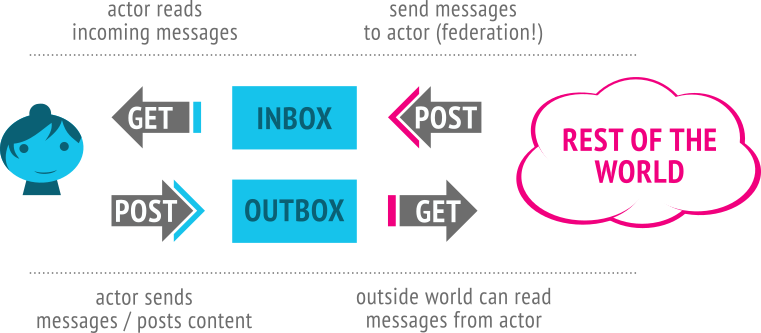
\includegraphics[width=\textwidth]{related_work/ActivityPub-tutorial-image.png}
  \caption{ActivityPub overview \cite{lemmer-webber_tallon_guy_prodromou_2018}}
  \label{fig:ap_flow}
\end{figure}
\pagebreak

Regarding security, ActivityPub's specification does not define any official security mechanisms to ensure confidentiality, non-repudiation, message integrity, authentication, or authorization \cite{lemmer-webber_tallon_guy_prodromou_2018}. It recommends using HTTPS for its HTTP-based communication, relying on third-party certificate authorities to provide transport-layer security. Nonetheless, other security aspects remain unaddressed. 


Although not included in ActivityPub, the SocialWG published a list of best security practices\footnote{https://www.w3.org/wiki/SocialCG/ActivityPub/Authentication\_Authorization} which suggests using standards like OAuth 2.0\footnote{https://oauth.net/2/} for client-to-server authentication, as well as HTTP Signatures\footnote{https://tools.ietf.org/html/draft-cavage-http-signatures-08} and Linked Data Signatures\footnote{https://w3c-dvcg.github.io/ld-signatures/} for server-to-server authentication.

HTTP signatures extend the HTTP protocol by adding the possibility to cryptographically sign the HTTP requests. This signature gets added to the request within the \emph{Signature} header, and it provides not only end-to-end message integrity but also proof of the authenticity of the sender without the need for multiple round-trips \cite{cavage_sporny_2019}. Following the same idea, Linked Data Signatures offer a way to create and attach signatures to JSON-LD documents, thus providing non-repudiation to e.g. an ActivityStreams Activity object even if the object has been shared, forwarded, or referenced at a future time \cite{celik_prodromou_le_hors_2014}.

The reason why these security specifications were not included in ActivityPub is unclear. Nonetheless, some ActivityPub-based social networks have added HTTP and JSON-LD signatures to their implementation. Providing a new layer of security for its userbase. One of these social networks is Mastodon, which will be explained in the next section.


% ------------ActivityPub-Based social networks------------------------------------
\section{ActivityPub-based Social Networks}

It is impossible not to refer to the \emph{Fediverse} when we talk about ActivityPub. The \emph{Fediverse} is an interoperable collection of different federated social networks running on free open software on thousands of servers across the world that implement the same open-standard protocols to be able to interact with each other. In today's most popular social networks like Facebook, Twitter, or Youtube, a centralized architecture keeps millions of users on one platform. Control, decision-making, user data, and censorship depend on a single profit-driven organization. On the contrary, the \emph{Fediverse} is developed by a not-profit-driven community of people around the globe independent of any corporation or official institution \cite{holloway_2018} \cite{https://doi.org/10.48550/arxiv.1909.05801}. The simplest way to explain how the federation works is the following example: Bob has a Twitter account, which he uses to follow all his friends that also have a Twitter account. Alice is a friend of Bob, but she only has an account on Youtube. In the real world, these two services are completely isolated and cannot communicate with each other. However, if both had implemented the same social network protocol, such as ActivityPub, Bob would be able to find Alice by a normal search on Twitter and follow her. Allowing any new post of Alice on Youtube, to appear in Bob's Twitter timeline.

Before ActivityPub, the \emph{Fediverse} implemented other protocols like \emph{Ostatus}\footnote{https://www.w3.org/community/ostatus/wiki/images/9/93/OStatus\_1.0\_Draft\_2.pdf}, \emph{Matrix}\footnote{https://matrix.org/}, and \emph{Diaspora}\footnote{https://diaspora.github.io/diaspora\_federation/}. However, after ActivityPub was published as a Recommendation by the SocialWG in January 2018, a big number of these federated social networks upgraded to ActivityPub. Becoming rapidly the predominant protocol. Furthermore, the range of services that can be found inside the \emph{Fediverse} includes blogging, microblogging, video streaming, photo, music sharing as well as file hosting. For example: 

\begin{itemize}
  \item \textbf{PeerTube\footnote{https://joinpeertube.org/}:} A decentralized alternative to video platforms, similar to Youtube.
  \item \textbf{Mastodon\footnote{https://joinmastodon.org/}:} A microblogging social network, similar to Twitter. 
  \item \textbf{Pixelfed\footnote{https://pixelfed.org//}:} An image-sharing platform, similar to Instagram. 
\end{itemize} 

Although it was not the first social network to implement ActivityPub, Mastodon is the one that pioneered its use on a large scale \cite{lemmer-webber_2017}. Moreover, it is still the social network in the \emph{Fediverse} with the biggest user base and popularity. For this reason, Mastodon will be used in this thesis as the representative of the ActivityPub-based social networks and will be explained further in the next section. 

% ------------Mastodon------------------------------------
\subsection{Mastodon}\label{subsec:mastodon}

 Mastodon is a decentralized microblogging social network created with the idea to bring social networking back into the hands of its users. The german creator of Mastodon, Eugen Rochko, shared the same opinion as what Fitzpatrick and Recordon said in 2007 \cite{fitzpatrick_recordon_2007}: \emph{People are getting sick of registering and re-declaring their friends on every site}. For this reason, Eugen envisioned a social network that could end this, and \emph{last forever} \cite{tilley_2018}. Similar to the \emph{Fediverse}, Mastodon differs from other commercial social networks in two aspects. First, it is oriented towards small communities and community-based services. Each \emph{instance}\footnote{A server running Mastodon} is free to choose its topics, this way users are encouraged to choose the instance better suited to their taste. Second, the Mastodon platform eliminates the presence of sponsored users or posts in feeds. This implies that the only way to connect or consume content is through a self-search to find an already known account or to explore the feeds of the users in other instances with similar interests \cite{8845221}. From a user experience perspective, Mastodon includes all the essential features of a microblogging platform, such as Twitter. This includes: 

\begin{itemize}
  \item Follow other users, even if they are not in the same instance. 
  \item Post small status updates, or \emph{toots}, up to 500 characters long. 
  \item Timeline of the local-instance and federated statuses. 
  \item Control over the visibility of their posts, with the option to set them as private, instance-level only, or federated. 
\end{itemize}


\cite{nottingham_2019}
As per documentation, Mastodon implements the following 4 different well-known endpoints: 

% \subsubsection{Change password}
% This endpoint origins form the proposal of the Web Application Security Working Group (WebAppSec) from the W3C, whose main mission is to provide security and policy frameworks to increase web application security and enable safe cross-site communication (https://www.w3.org/groups/wg/). It defines a well-known URL that sites can use to make their change password forms discoverable by tools. This URL would enable software, specially password managers, to easily redirect users to the right link for them to change their password.

% \subsubsection{NodeInfo}
% NodeInfo is an initiative to standardize the presentation of metadata about a server operating one of the distributed social networks. The two main aims are to get greater insights into the distributed social networking user base and to provide tools that allow users to select the most suited software and server for their requirements. Mastodon is one of the implementers of this protocol, along with other federated social networks such as Diaspora, Peertube and WordPress [http://nodeinfo.diaspora.software/ ]. NodeInfo specifies that servers must provide the well-known path /.well-known/nodeinfo and provide a JRD document referencing the supported documents via Link elements, as shown in \label{NodeInfo response example}. [http://nodeinfo.diaspora.software/protocol.html ] Accessing the hypertext reference from the JRD response will give a schematized series of metadata of the instance running the endpoint, such as NodeInfo schema version, software, protocols supported by the server, statistics and even a list of third-party services that can interact with the server via an API. Figure \label{fig:nodeinfo_response} shows the NodeInfo 2.0 schema of the Mastodon instance mastodon.social. 

\lstset{style=JSONStyle}
\begin{lstlisting}[caption=NodeInfo response example, label=NodeInfo response example, float=h]
  {
      "links": [
          {
            "rel": "http://nodeinfo.diaspora.software/ns/schema/2.1",
              "href": "https://example.org/nodeinfo/2.1"
          }
      ]
  }
\end{lstlisting}

\lstset{style=JSONStyle}
\begin{lstlisting}[language=PHP, caption=NodeInfo request]
    GET /wel-known/nodeinfo/2.0 HTTP/1.1
    Host: mastodon.social
\end{lstlisting}

\lstset{style=JSONStyle}
\begin{lstlisting}[language=PHP, caption=NodeInfo response for mastodon.social, label=fig:nodeinfo_response, float=h]
{
   "version": "2.0",
   "software": {
       "name": "mastodon",
       "version": "3.5.3"
   },
   "protocols": [
       "activitypub"
   ],
   "services": {
       "outbound": [],
       "inbound": []
   },
   "usage": {
       "users": {
           "total": 718555,
           "activeMonth": 61717,
           "activeHalfyear": 178356
       },
       "localPosts": 36484017
   },
   "openRegistrations": true,
   "metadata": []
}
\end{lstlisting}


\subsubsection{Web Host Metadata}
    Web host metadata is a lightweight metadata document format that allows for the identification of host policy or information, where \emph{host} refers to the entity in charge of a collection of resources defined by URIs with a common URI host. It employs the XRD 1.0\footnote{https://docs.oasis-open.org/xri/xrd/v1.0/os/xrd-1.0-os.html} document format, which offers a basic and flexible XML-based schema for resource description. Moreover, it provides two mechanisms for providing resource-specific information, specifically,  \emph{link templates} and \emph{Link-based Resource Descriptor Documents} (LRDD). On the one hand, link templates require a URI to work, thus avoiding the use of fixed URIs. On the other hand, the LRDD relation type is used to relate LRDD documents to resources or host-meta documents \cite{cook_2011}. In the specific case of the Mastodon implementation, requesting the host-meta endpoint will give us back the \emph{lrdd} link to the Webfinger endpoint, where specific resource information can be found. This is illustrated by figures \ref{fig:host_metadata_response} and \ref{fig:host_metadata_request}.

\lstset{style=JSONStyle}
\begin{lstlisting}[language=PHP, caption=Example Host Metadata request to mastodon.social, label=fig:host_metadata_request, float=h]
    GET /.well-known/host-meta HTTP/1.1
    Host: mastodon.social
    Accept: application/xrd+xml
\end{lstlisting}

\lstset{style=JSONStyle}
\begin{lstlisting}[language=XML, caption=Example Host metadata response from mastodon.social, label=fig:host_metadata_response, float=h!]
    <?xml version="1.0" encoding="UTF-8"?>
    <XRD xmlns="http://docs.oasis-open.org/ns/xri/xrd-1.0">
      <Link rel="lrdd" template="https://mastodon.social/.well-known/webfinger?resource={uri}"/>
    </XRD>
\end{lstlisting}

\subsubsection{Webfinger}
Finally, Webfinger is the protocol on which Mastodon heavily relies for the resolving process and its federated functioning \cite{rochko_2020}. Webfinger allows for discovering information about persons or other entities on the Internet using HTTP such as a personal profile address, identity service, telephone number or email. Performing a query to a WebFinger endpoint requires a query component with a resource parameter, which is the URI that identifies the identity that is being looked up. Mastodon employs the \emph{acct}\footnote{https://datatracker.ietf.org/doc/html/rfc7565} URI format, which aims to offer a scheme that generically identifies a user's account with a service provider without requiring a specific protocol. In the same way NodeInfo works, it returns a JRD Document describing the entity \cite{jones_salgueiro_jones_smarr_2013}.  Fig. \label{Webfinger response from mastodon.social} shows an example of the returned JRD that is being provided by the WebFinger endpoint in the mastodon social instance when querying the account "acct:bob@mastodon.social".

\lstset{style=JSONStyle}
\begin{lstlisting}[language=PHP, caption=HTTP request to Webfinger endpoint, label=Webfinger request, float=h]
  GET /.well-known/webfinger?resource=acct:bob@mastodon.social
  Host: mastodon.social
  Accept: application/xrd+xml
\end{lstlisting}

\lstset{style=JSONStyle}
\begin{lstlisting}[language=PHP, caption=Webfinger response, label=Webfinger response from mastodon.social, float=h]
{
   "subject": "acct:bob@mastodon.social",
   "aliases": [
       "https://mastodon.social/@bob",
       "https://mastodon.social/users/bob"
   ],
   "links": [
       {
           "rel": "http://webfinger.net/rel/profile-page",
           "type": "text/html",
           "href": "https://mastodon.social/@bob"
       },
       {
           "rel": "self",
           "type": "application/activity+json",
           "href": "https://mastodon.social/users/bob"
       },
       {
           "rel": "http://ostatus.org/schema/1.0/subscribe",
           "template": "https://mastodon.social/authorize_interaction?uri={uri}"
       }
   ]
}
\end{lstlisting}


\section{Decentralized Identifiers} \label{section:dids}

Globally unique identifiers are used by individuals, organizations, abstract entities, and even internet of things devices for all kinds of different contexts. Nonetheless, the large majority of these globally unique identifiers are not under the entity's control. We rely on external authorities to issue them, allowing them to decide who or what they refer to and when they can be revoked. Their existence, validity scope and even the security mechanisms that protect them are all dependent on these external authorities. Leaving their actual owners helpless against any kind of threat or misuse \cite{sporny_longley_sabadello_reed_steele_2021}. In order to address this lack of control, the W3C DID Working Group conceptualized the Decentralized Identifiers or \emph{DIDs}.

DIDs are a new type of globally unique identifier that enables individuals and organizations to create their own identifiers using trustworthy systems. By means of this, entities are able to prove control over them by authenticating using cryptographic proofs. Furthermore, given that the generation and assertion of DIDs are entity-controlled, an entity can create any number of DIDs that can be tailored and confined to specific contexts. This would enable interaction with other systems, institutions, or entities that require authentication while also limiting the amount of personal or private data to be revealed. All of this without the need to rely on a central authority \cite{sporny_longley_sabadello_reed_steele_2021}. To better illustrate how DIDs work, let's address the components which constitute DIDs. Figure \ref{fig:did_architecture} provides a basic overview of the major components of the Decentralized Identifier architecture.

\begin{figure}[H]
  \centering
  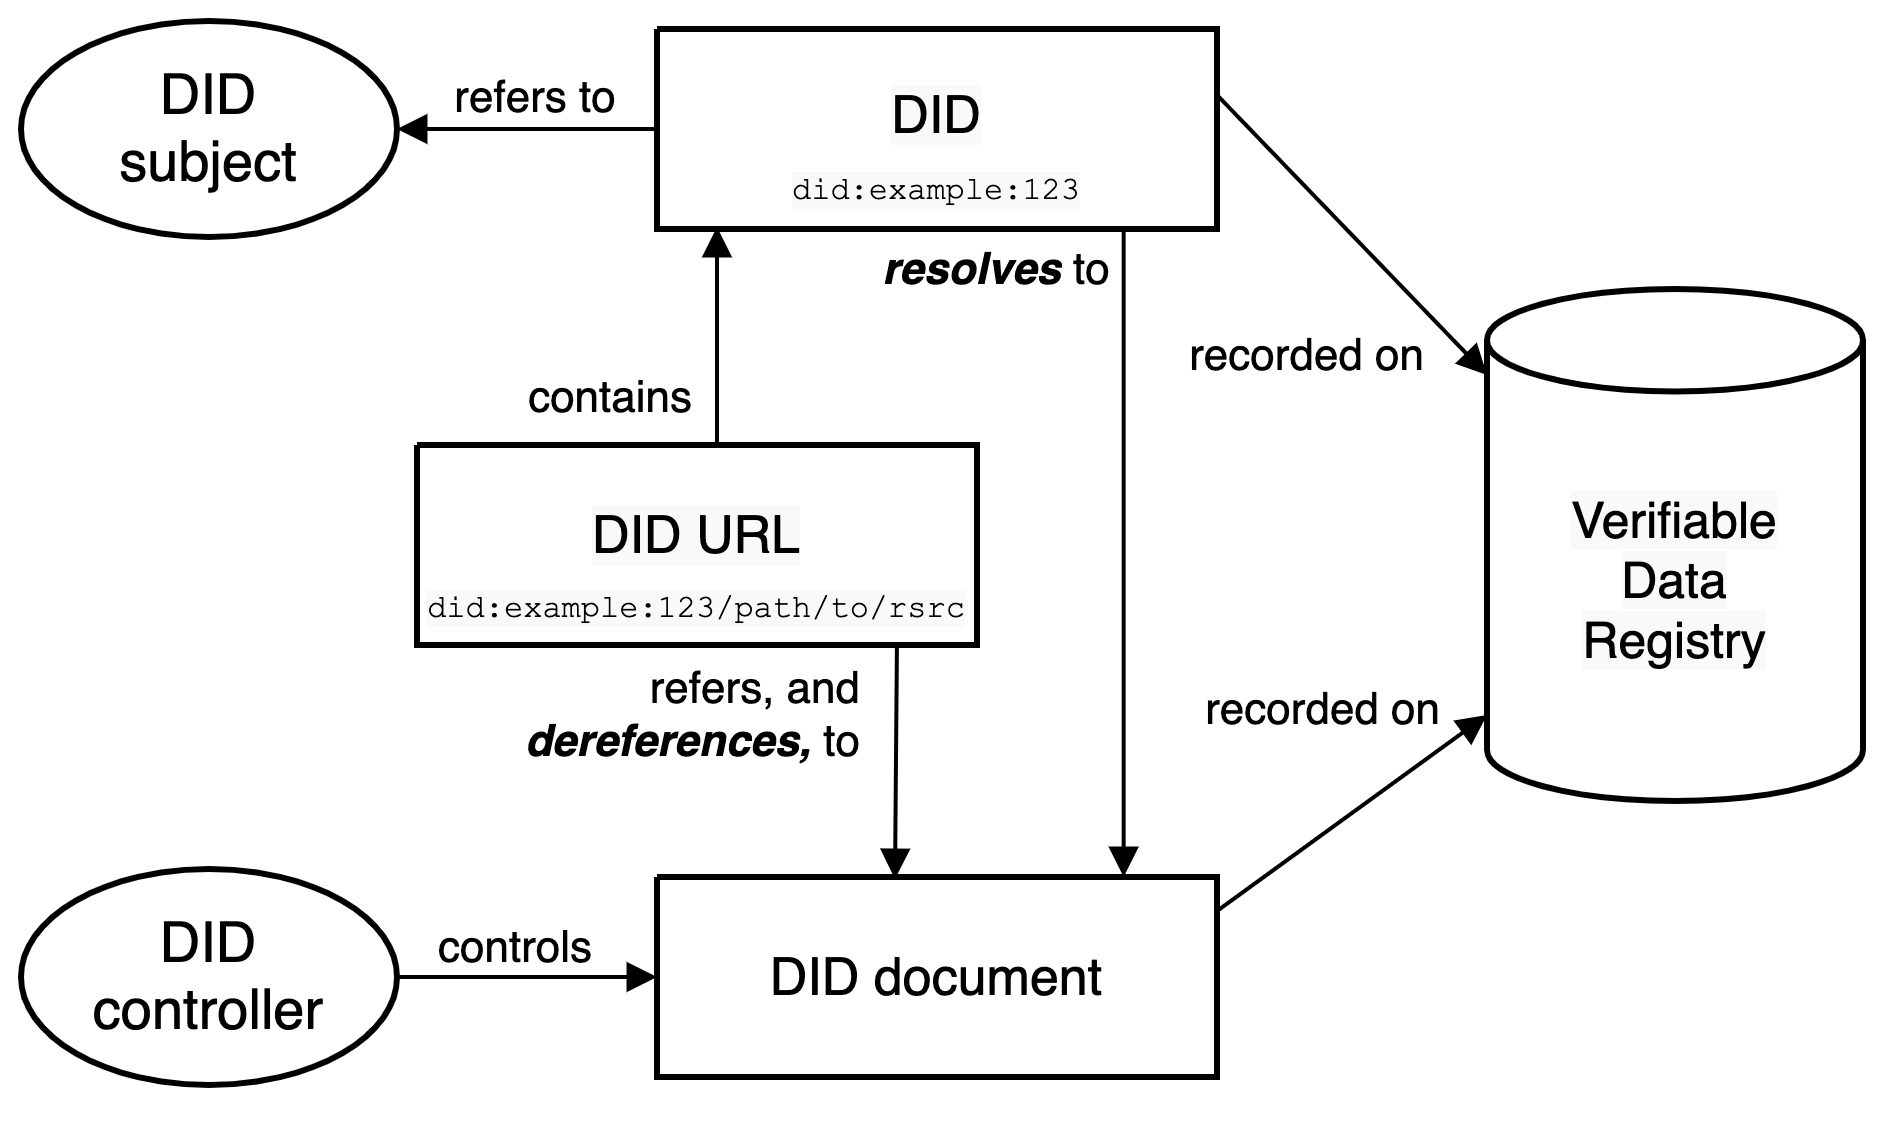
\includegraphics[width=\textwidth]{related_work/did_brief_architecture_overview.png}
  \caption{DID architecture overview \cite{sporny_longley_sabadello_reed_steele_2021}}
  \label{fig:did_architecture}
\end{figure}

\subsection{DID}  
The DID itself is a URI\footnote{https://www.rfc-editor.org/rfc/rfc3986} that consists of 3 different parts, namely the did URI scheme identifier, the method identifier and the DID method-specific identifier.

\begin{figure}[h]
  \centering
  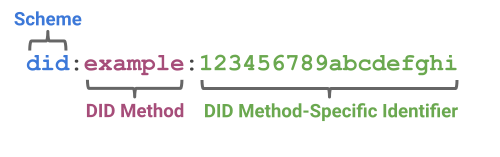
\includegraphics[width=\textwidth]{related_work/parts-of-a-did.png}
  \caption{DID composition \cite{sporny_longley_sabadello_reed_steele_2021}}
  \label{fig:did}
\end{figure}

\subsection{DID URL}

A DID can include a path, query and fragment to be able to locate a specific resource inside a DID document, as shown in \ref{fig:did_architecture}


\subsection{DID Subject}

Refers to the entity being identified by the DID. According to the specification \cite{sporny_longley_sabadello_reed_steele_2021}, any person, group, organization, physical thing, digital thing or logical thing can be a DID Subject.

\subsection{DID Controller}

The DID controller is the entity that can make changes to the DID Document. This entity is not necessarily the DID Subject itself.
  
\subsection{DID Document}

They contain information associated with a DID. They usually describe verification methods, such as cryptographic public keys, as well as services that are relevant to interactions with the DID Subject. An example of a DID Document can be seen in \ref{fig:did_document}.

\lstset{style=JSONStyle}
\begin{lstlisting}[language=PHP, caption=Example DID Document, label=fig:did_document]
{
  "@context": "https://w3id.org/did/v1",
  "id": "did:example:123456789abcdefghi",
  "publicKey": [{
    "id": "did:example:123456789abcdefghi#keys-1",
    "type": "RsaVerificationKey2018",
    "owner": "did:example:123456789abcdefghi",
    "publicKeyPem": "..."
  }],
  "authentication": [{
    "type": "RsaSignatureAuthentication2018",
    "publicKey": "did:example:123456789abcdefghi#keys-1"
  }],
  "service": [{
    "type": "ExampleService",
    "serviceEndpoint": "https://example.com/endpoint/8377464"
  }]
}

% \end{lstlisting}

The only required attribute for a DID Document is the ID. Other optional attributes include a controller, which specifies the DID Controller; verification methods, used to authenticate or authorize interactions with the DID subject or associated parties; and services, which can be any type of service the DID subject wants to advertise, including decentralized identity management services for further discovery, authentication, authorization, or interaction.
 

\subsection{DID methods}

DID methods describe the processes for CRUD operations for DIDs and DID documents, based on a specific type of verifiable data registry. Each DID method describes and implements its own security and privacy considerations. According to the DID registry of the W3C\footnote{https://www.w3.org/TR/did-spec-registries/\#did-methods}, there are around 130 registered DID methods. Based on their characteristics and patterns, the following 4-way classification of DIDs has arisen.

\begin{itemize}
  \item \textbf{Ledger-based DIDs}: This includes all the DIDs that store DIDs in a blockchain or other Distributed Ledger Technologies (DLTs). Examples include did:btcr, did:ethr and did:trx, whose DIDs are stored correspondingly in the Bitcoin, Ethereum and Tron network \cite{preukschat_reed_2021}.
  % \item \textbf{Ledger Middleware ("Layer 2") DIDs}: Broadly speaking, Layer 2 refers to a framework or protocol that is built on top of an existing blockchain system that takes the transactional burden away from layer 1 and post-finalized proofs back to layer 1. By removing this transaction load from layer 1, the base layer becomes less congested, and everything becomes more scalable [https://ethereum.org/en/layer-2/ ]. The Lightning Network ( \, LN	) \, is an example of a layer 2 Bitcoin protocol that offers users a fast micro-payment platform. Furthermore, regarding Layer 2 DID methods, the DIF has developed Sidetree\footnote{https://github.com/decentralized-identity/sidetree}. A protocol for creating scalable blockchain-agnostic Decentralized Identifier networks that enable users to create globally unique, user-controlled identifiers and manage their associated PKI metadata, without the need for centralized authorities or trusted third parties \cite{buchner_steele_ronda_2021}.
  Examples include: did:ion, did:elem.
  \item \textbf{Peer DIDs}: DIDs have the required ability to be resolvable, however not all of them have to be globally resolvable. The DIDs in this category do not exist on a global source of truth but in the context of relationships between peers in a limited number of participants. Nonetheless, their validity is not affected since they comply with the core properties and functionalities that a DID has to provide. 

  \item \textbf{Static DIDs}: This type of DIDs are limited in the kind of operations that can be performed on them. These DIDs are not stored in any registry, consequently, it is not possible to update, deactivate or rotate them. Using the did:key method as an example, the DID-method-specific part of the DID is encoded in a way that the DID document can be deterministically extracted from the DID itself \cite{longley_zagidulin_sporny_2022}.
\end{itemize}


did:ethr
This DID method was registered by Uport, an Ethereum-based system for self-sovereign identity \cite{Lundkvist_Heck_Torstensson_Mitton_Sena_2016}. It allows any Ethereum smart contract or key pair account, or any secp256k1 public key to becoming a valid identifier \cite{nistor_grassberger_carlin_2022}. UPort is a smart-contract-based system that abstracts user accounts using proxy contracts that are held by the user but may be retrieved if keys are lost. To do this, controller contracts create trusted entities for asserting ownership \cite{8783188}


did:ens:
% The Ethereum Name Service (ENS) is a distributed, open, and extensible naming system based on the Ethereum blockchain. Its purpose is to map names like 'bob.eth' into machine-readable identifiers like Ethereum addresses, other cryptocurrency addresses, content hashes, and metadata. In the same way the Domain Name System (DNS) maps human-readable domains like 'google.com' to IP addresses. However, their architecture differs due to the capabilities and constraints of the Ethereum blockchain. (https://github.com/veramolabs/did-ens-spec )
% This DID method was registered by Consensys, a blockchain venture studio founded by Ethereum's cofounder Joseph Lubin that supports Ethereum-based projects. Some of these projects include uPort, Metamask, Civil, Truffle and Gnosis. [https://decrypt.co/resources/consensys]. 


% This DID method was created with the following objectives, firstly to integrate ENS names to be interoperable with applications that implement DIDs, and secondly, to add DID-capabilities to ENS names such as services and verification methods [https://github.com/veramolabs/did-ens-spec].

% did:ion:
% This DID method works by registering DIDs to the Bitcoin network. Launched to the public in March 2021, Identity Overlay Network (ION) is Microsoft's DID-network built on top of the Bitcoin Network implemented using Sidetree (https://techcommunity.microsoft.com/t5/identity-standards-blog/ion-we-have-liftoff/ba-p/1441555 ). 
% ION is public, permissionless, it does not implement its own currency and its nodes do not require an additional consensus mechanism. (https://github.com/decentralized-identity/ion ).

\subsection{Verifiable Data Registry}

Essentially, any system that enables capturing DIDs and returning required data to generate DID documents. This can be distributed ledgers, decentralized file systems, any type of database, peer-to-peer networks, or other types of trustworthy data storage \cite{sporny_longley_sabadello_reed_steele_2021}.

\subsection{DID resolver}

A DID resolver is able to implement the DID resolution, which consists of taking a DID as an input, and giving a DID Document as an output \cite{sporny_longley_sabadello_reed_steele_2021}. As of the writing of this thesis, the Identifiers \& Discovery Working Group (ID WG) has implemented a prototype Universal Resolver\footnote{https://github.com/decentralized-identity/universal-resolver}, which allows the resolution of DIDs for numerous DID methods, including all the examples mentioned above. In addition, this working group has also developed a Universal Registrar\footnote{https://uniregistrar.io/}, which allows the creation, edition and deactivation of the DIDs across different DID methods.

% Comparing DIDs with other identifiers


% UUID Universally Unique Identifiers: 
% UUIDs are similar to DIDs, because they do not require a centralized registration authority. But they are not resolvable or cryptographically-verifiable. 


% Almost all types of identifier systems can support DIDs. This would create an interoperability bridge between centralized, federated and decentralized worlds. Implementers can use any kind of computing infrastructure they trust, such as distributed ledgers, decentralized file systems, distributed databases or peer-to-peer networks. 


% Services
% Services are used to specify ways to communicate with the DID subject. Services can be decentralized identity management for further discovery, authentication, authorization or interaction. 


% DID Privacy 

% The 7 Principles of Privacy by design have been applied to DIDs. (https://iapp.org/media/pdf/resource_center/pbd_implement_7found_principles.pdf )






%  A DID is unlikely to contain any information about the DID subject, so further information about the DID subject is only discoverable by resolving the DID to the DID document, obtaining a verifiable credential about the DID, or via some other description of the DID.



\section{DIDComm Messaging}\label{section:didcomm}

\subsection{Definition}

The Hyperledger Foundation is an open-source collaborative effort intended to further develop blockchain technologies across industries \cite{jones_boswell_2022}. Started in 2016 by the Linux Foundation, it has given birth to numerous enterprise-grade software open-source projects that can be classified into DLTs, libraries, tools and labs \cite{lusard_lehors_muscara_boswell_zsigri_2021}. One of these graduate projects is Hyperledger Aries, which together with Hyperledger Indy (HI) and Hyperledger Ursa (HU), makes up the Sovereign Identity Blockchain Solutions of Hyperledger. HI supplies a distributed ledger specifically built for decentralized identity, HU is a shared cryptography library that helps to avoid duplicating cryptographic work across projects while also potentially increasing security. Finally, Aries provides solutions for SSI-based identity management, including key management, credential management, and an encrypted, peer-to-peer DID-based messaging system that is now labeled as Didcomm v1 \cite{jones_boswell_2022}. 
Based on Didcomm v1, the Communication Working Group (CWG) of the DIF has implemented DIDcomm v2. Among other key differences between versions, such as formalizations of Didcomm v1 methods, Didcomm v2 has removed the special handling of Peer-DIDs in order to make all DIDs equal from the perspective of the DIDComm spec. Furthermore, the CWG pursues the standardization of DIDcomm not only to widen its implementation beyond Aries-based projects but to create an interoperable layer that would allow higher-order protocols to build upon its security, privacy, decentralization, and transport independence in the same way web services build upon HTTP. \cite{young_2020} \cite{curren_looker_terbu_2020}

From this point on, we are going to refer to DIDComm Messaging v2 only as DIDComm. Didcomm can be described as a communication protocol that promises a secure and private methodology that builds on top of the decentralized design of DIDs. Moreover, Didcomm is a very versatile protocol, as it supports a wide range of features, such as security, privacy, decentralization, routable, interoperability, and the ability to be transport-agnostic \cite{curren_looker_terbu_2020}.

To better understand how it works, let's look at how it would work in a scenario where Alice wants to send a private message to Bob: 


% \begin{algorithm}[H]
% \caption{Example of DID communication using DIDComm \cite{Abramson_2020}}
% \label{alg:didcomm_example}
%   \begin{algorithmic}[1]
%     \State Alice has a private key \emph{sk\textsubscript{a}} and a DID Document for Bob containing an endpoint \emph{(endpoint\textsubscript{bob})} and a public key \emph{(pk\textsubscript{b})}.

%     \State Bob has a private key \emph{sk\textsubscript{b}} and a DID Document for Alice containing her public key \emph{(pk\textsubscript{a})}.

%     \State Alice encrypts plaintext message \emph{(m)} using pk\textsubscript{b} and creates an encrypted message \emph{(eb)}.

%     \State Alice signs eb using her private key \emph{sk\textsubscript{a}} and creates a signature \emph{(s)}.

%     \State Alice sends \emph{(eb, s)} to \emph{endpoint\textsubscript{bob}}.

%     \State Bob receives the message from Alice at \emph{{endpoint\textsubscript{bob}}.}

%     \State Bob verifies \emph{(s)} using Alice's public key \emph{pk\textsubscript{a}}

%     \If{Verify \emph{(eb, s, pk\textsubscript{a})} = 1}
%     \State Bob decrypts \emph{eb} using \emph{sk\textsubscript{b}}.
%     \State Bob reads the plaintext message \emph{(m)} sent by Alice
%     \EndIf
%   \end{algorithmic}
% \end{algorithm}


% [https://arxiv.org/pdf/2006.02456.pdf ]

DIDComm differs from the current dominant web paradigm, where something as simple as an API call requires an almost immediate response through the same channel from the receiving end. This duplex request-response interaction is, however, not always possible as many agents may not have a constant network connection or may interact only in larger time frames, or may even not listen over the same channel where the original message was sent. DIDComm's paradigm is asynchronous and \emph{simplex}. Thus showing a bigger resemblance with the email paradigm. Furthermore, the web paradigm goes under the assumption that traditional methods for processes like authentication, session management, and end-to-end encryption are being used. Didcomm does not require certificates from external parties to establish trust, nor does it require constant connections for end-to-end transport-level encryption (TLS). Taking the security and privacy responsibility away from institutions and placing it with the agents. All of this without limiting the communication possibilities because of its ability to function as a base layer where opposed capabilities like sessions and synchronous interactions can be built upon. \cite{curren_looker_terbu_2020}

To achieve the encryption and signing processes mentioned in algorithm \ref{alg:didcomm_example}, Didcomm implements a family of the Internet Engineering Task Force (IETF) standards, collectively called JSON Object Signing and Encryption (JOSE), which will be further explained in the next section. 

\subsection{JOSE Family}

This RFC family includes both the JSON Web Signature (JWS) and the JSON Web Encryption (JWE) standards that are subclasses of the JSON Web Token (JWT), and JSON Web Key (JWK).


The second part of the DIDComm enablement, namely the signing and encrypting, will depend on what kind of security guarantees we want to achieve. DIDComm offers different approaches based on signing and two types of message encryption. Authenticated Sender Encryption (\emph{authcrypt}) and Anonymous Sender Encryption (\emph{anoncrypt}) are both encrypted and delivered to the recipient's DID. Still, they differ because only \emph{authcrypt} gives direct guarantees about the sender's identity. Sending anonymous messages in social networks is not usually the case, and removing the attribution of a post can lead to other problems \cite{martin_2022}. However, social networks like Ask.fm\footnote{https//ask.fm} or NGL\footnote{https://ask.fun} that rely on anonymous posts could use the advantages of \emph{anoncrypt}.

DIDComm recommends using \emph{authcrypt} as the standard to provide confidentiality, message integrity, and authenticity of the sender. For this, \emph{authcrypt} requires the public key authenticated encryption algorithm \emph{ECDH-1PU}\footnote{https://datatracker.ietf.org/doc/html/draft-madden-jose-ecdh-1pu-04}. This algorithm j

This is due to the use of the 
Elliptic-curve Diffie\-Hellman (ECDH) protocol, which allows two parties to build a secure and private channel across an insecure and observable network. This protocol is part of the foundation of popular messaging apps such as Facebook Messenger, Whatsapp, Signal, and Didcomm V1 \cite{shaaban_2021}. This key agreement protocol works by having both parties interchanging the public keys of their EC keypairs and some other public information. Using this public data and their private keys both parties can calculate a shared secret value, which it's the same for both parties. Any other observer or third party is not able to compute this shared secret without the private data \cite{5972416}. 

An alternative to \emph{Authcrypt} that also complies with the required confidentiality and non-repudiation requirements is to have a nested JWT. To achieve this, the plaintext is first signed and then the resulting JWS is used as the payload of a JWE. The algorithm \ref{alg:nested_jwt} illustrates better the workings of this. 

\begin{algorithm}[H]
  \caption{Communication example with nested JWT}
  \label{alg:nested_jwt}
    \begin{algorithmic}[1]
      \State Alice signs a plain text message using her private key \emph{sk\textsubscript{a}} and creates a \emph{(jws)}.
  
      \State Alice encrypts the \emph{(jws)} using Bob's public key pk\textsubscript{b} and creates a \emph{(jwe)}.
  
      \State Alice sends \emph{jwe} to Bob.
  
      \State Bob decrypts \emph{(jwe)} using his private key \emph{sk\textsubscript{b}} and obtains the \emph{jws}
      \State Bob verifies \emph{(jws)} using Alice's public key \emph{pk\textsubscript{a}}
  \end{algorithmic}
\end{algorithm}
  
In both alternatives, the identity of the sender can be confirmed and the plain text message remains encrypted and hidden from any third party that might manage to read the payload. As mentioned in \autoref{section:didcomm}, the JWE can be sent through any unprotected protocol and still keep all of its advantages. 



Compare with other encryption methods. (TLS, Whatsapp end-to-end, Signal) (Use image below)
 